\documentclass[12pt]{beamer}
\usetheme{Boadilla}
\usepackage{graphicx}
\usepackage{algorithm2e}
\graphicspath{{images/}}
\title{CMPT 155: Computer Applications for Life Sciences}
\subtitle{Lecture 9:  Regression}
\author{Ivan E. Perez}
\date{March 4, 2022}
\usepackage{booktabs} % Allows the use of \toprule, 
\usepackage{appendix}
\usepackage{enumerate,multicol}
\usepackage{amsmath, amssymb, amsthm}
\usepackage{tikz}
\usepackage{amsxtra}
\begin{document}
	
	\begin{frame}
		\titlepage
	\end{frame}
	
	\begin{frame}
		\frametitle{Presentation Outline}
		\tableofcontents
	\end{frame}
	\section{Administrative}
	\begin{frame}
		\frametitle{Homework And Administrative}
		\begin{itemize}
			\item Midterm 2 is on April $13^{\text{th}}$.
			\item You may bring a 1 page cheat sheet print or handwritten. 
			\item Homework 5 is due ???
		\end{itemize}
	\end{frame}
	\begin{frame}
		\frametitle{Trendline (Regression Line)}
		\begin{itemize}
			\item Data analysis is about revealing patterns and facts about data sets.
			\item Linear regression is a technique describes outputs $y$ as linearly dependent on inputs $x$.
		\end{itemize}
	\end{frame}
	
	\begin{frame}
		\frametitle{Trendline Example}
		\begin{center}
		\begin{figure}
		\includegraphics[width=0.9\textwidth]{RegressionExample.png}
		\caption{Example Linear Regression of Age against Reflex Time}
		\end{figure}
		\end{center}
	\end{frame}

	\begin{frame}
		\frametitle{Adding a Trendline}
		A Trendline can be added to XY (Scatter) graphs. \\
		Lets try plotting \textit{CancerStudy.xlsx} and adding a Trendline:
		\begin{enumerate}
			\item Download \textit{CancerStudy.xlsx} from moodle.
			\item Select cells \texttt{B2:C18}
			\item Navigate to the XY Scatter Plot, and create scatter plot.
			\item be sure to include a chart title and axis titles.
			\item To add a trendline we can:
				\begin{itemize}
					\item `Chart Tools' $\rightarrow$ `Add Chart Element' $\rightarrow$ `Linear'.
					\item Select the Datapoints $\rightarrow$ right(Ctrl)-click $\rightarrow$ `Add Trendline'
				\end{itemize}
		\end{enumerate}
	\end{frame}

	\begin{frame}
		\frametitle{Types of Trendlines}
		\begin{center}
		\begin{tabular}{l  |l   |l  }
			Type & Excel Option & General Form \\
			\hline
			Linear & Linear & $y=mx+b$\\
			Exponential &  Exponential & $y=ae^{bx}$\\
			Quadratic & Polynomial deg=2 & $y=ax^2 + bx+ c$\\
			Cubic & Polynomial deg=3 & $y=ax^3 + bx^2 + cx + d$
		\end{tabular}
		\end{center}
		When computing predictions in excel, we can write trendline equations in the following fashion.
		\begin{center}
		\begin{tabular}{l | l} 
		Type & Excel Form\\
		\hline
		Linear & \texttt{m * X + b}\\
		Exponential& \texttt{(a)*EXP((b)*x)}\\
		Quadratic & \texttt{(a)*(X$\wedge$2) + (b)*X + c}\\
		Cubic & \texttt{(a)*(X$\wedge$3) +(b)*(X$\wedge$2) + (c)*X} + d\\
		\end{tabular}
		\end{center}
		Where \texttt{X} is a \textit{cell reference} to an $x$-value in the dataset and \texttt{a,b,c,d, m} are real numbers that can be written as a decimal or in 
		scientific notation $1.234 * 10^{-4}$, (i.e., \texttt{1.234 * (10$\wedge$-4)})
	\end{frame}

	\begin{frame}
		\frametitle{Formatting Trendlines}
		Trendlines can be formatted through the `Format Trendline' pane, which can be accessed by:
		\begin{enumerate}
			\item Selecting Data by left clicking a point on the XY scatter graph.
			\item Right(Ctrl) clicking the points
			\item Selecting the `Format Trendline' menu option.
		\end{enumerate} 
	\bigskip
		Trendlines modifitcations include:
			\begin{itemize}
				\item Equation and Displayed Statistics.
					\begin{itemize}
						\item The equation of the trendline
						\item whether to display the equation
						\item whether to display correlation squared, $\text{R}^2$. 
					\end{itemize} 
				\item Thickness and color
					\begin{itemize}
						\item  Thickness, color, effects, labelling 
					\end{itemize}
				\item Extrapolation
					\begin{itemize}
						\item The range of the trendline is within the dataset by default
						\item can be extraoplated by increasing the Forward/Backward periods option
					\end{itemize}
		\end{itemize}
	\end{frame}
\section{Analyzing Trendlines}
	\begin{frame}
		\frametitle{Analyzing Trendlines}
		After specifying a model we must be able to specify, analyze and measure models. 
		Common functions for Analyzing a \textit{linear} trendline include:
		\begin{itemize}
			\item slope using SLOPE()
			\item $y$- intercept using INTERCEPT()
			\item Correlation, R,using CORRELL()
		\end{itemize}
		Non Linear Trendlines can be analyzed using \textit{Sum of Squared Residuals},SSR. 
	\end{frame}

	\begin{frame}
		\frametitle{SLOPE()}
		SLOPE()  - computes the slope of a linear regression line for a collection of $x$ and $y$ values. 
		\begin{itemize}
			\item inputs 
				\begin{itemize}
					 \item \texttt{known\_ys} : selection \\ 
					 array/selection of known $y$ values
					 \item \texttt{known\_xs : selection} \\
					 array/selection of known $x$ values
				\end{itemize}
			\item outputs 
				\begin{itemize}
					\item computed slope : numeric\\
					estimated slope for a linear regression line for the given data.
				\end{itemize}
			\end{itemize}
	\end{frame}
	\begin{frame}
		\frametitle{INTERCEPT()}
		Compute the $y$ intercept of a linear regression line for a collection of $x$ and $y$ values. 
		\begin{itemize}
			\item inputs 
			\begin{itemize}
				\item \texttt{known\_ys} : selection \\ 
				array/selection of known $y$ values
				\item \texttt{known\_xs} : selection \\
				array/selection of known $x$ values
			\end{itemize}
			\item outputs 
			\begin{itemize}
				\item computed intercept : numeric\\
				estimated \textbf{intercept} for a linear regression line for the given data.
			\end{itemize}
		\end{itemize}
	\end{frame}
	\begin{frame}
		\frametitle{Correlation Coefficeint (R)}
		Measures the correlations between $x$'s and $y$'s. 
		\begin{itemize}
			\item inputs : 
			\begin{itemize}
				\item \texttt{known\_x} : selection \\
				array/selection of known $x$'s.
				\item \texttt{known\_y} : selection \\
				array/selection of known $y$'s.
			\end{itemize}
		\item outputs :
			\begin{itemize}
				\item correlation : numeric \\
				correlation coeffecient; between -1 and 1. 
			\end{itemize}
		\end{itemize}
	
	\end{frame}

\begin{frame}
	\frametitle{Interpretting Correlation Coeffecients}
	\begin{tabular}{r | l }
		R value & Qualitative description\\
		\hline
		$-1 \leq \text{R}\leq-0.7$ & Very Strong Negative Correlation \\
		$-0.7<\text{R} \leq -0.4 $&  Strong Negative Correlation \\
		$-0.40 < \text{R} \leq -0.3$ & Moderate Negative relationship \\
		$-0.30 < \text{R} \leq -0.2 $ & weak positive relationship \\
		$-0.2 < \text{R} < 0  $&  no or negligiabel relationship\\
		$\text{R}=0$ & No relationship\\
		$0<\text{R} \leq 0.2 $& No or gelible relationship \\
		$0.2 < \text{R} \leq 0.3 $ &weak positive correlation \\
		$0.3 < \text{R} \leq 0.4$ &  moderate positive correlation \\
		$0.4 < \text{R} \leq 0.7$ & Strong positive correlation\\
		$0.7< \text{R} \leq 1$ & Very Strong Positive Correlation.
	\end{tabular}\\
	\bigskip
	Want to learn more for a correlation coeffecients? Check out
	\textcolor{blue}{
	\href{https://www.statisticshowto.com/probability-and-statistics/correlation-coefficient-formula/}{CorrelationCoefficient - StatisticsHowTo}}
\end{frame}
	\begin{frame}
		\frametitle{Which Trendline to choose?}
	Things to Consider:
	\begin{itemize}
		\item What kind of relationship do you expect between your datapoints?
		\item What are the limitations of this dataset?
			\begin{itemize}
				\item Do you expect to collect data outside this range?
				\item Is this survey of physical data?
			\end{itemize}
		\item How will this trendline be used in your later analysis?
		\item How do you measure best fit and trendline performance?	
\end{itemize}
	\end{frame}

	\begin{frame}
		\frametitle{Which Trendline to choose?}
		Common measures of trendline fit are 
		\begin{itemize}
			\item Pearsons $\text{R}^2$. 
			\begin{itemize}
				\item is equal to squared correlation
				\item can only be used with \textit{Linear} regression lines
			\end{itemize}
			\item Sum of Squared Residuals \textit{SSR}.
			\begin{itemize}
				\item Takes a sum of the \textit{square} of the \textcolor{red}{residuals} (i.e., difference between the actual data and estimated function value).
				\item the \color{red}{\textit{smaller}} the \textit{better} the trendline fit.  
			\end{itemize}
		\end{itemize}
	\end{frame}
\section{Prediction}
	\begin{frame}
		\frametitle{Prediction}
		\begin{itemize}
			\item Trendlines can be used to to predict values you don't have. 
				\begin{itemize}
					\item In Sample Predicition (interpolation) : Using the \textit{trendline} to predict values that fall within the range of sample data that was used to create the trendline.
					\item Out of Sample Predition(extrapolation) : Using the \textit{trendline} to predict values that fall out of the range of sample data that was used to create the trendline.
			\end{itemize}
		\item for Extrapolation, you can visualize these predictions by adding \textit{forward} and \textit{backward} periods to the trendline in the \textit{Format Trendline} panel.
	\end{itemize}
	\end{frame}

	\begin{frame}
		\frametitle{Prediciton}
		\begin{itemize}
			\item Lets try predicting the mortality in regions by:
				\begin{itemize}
					\item Interpolation :  average annual temperatures between 30 and 50 degrees, in 1 degree increments. 
					\item Extrapolating : average annual temperatures between 55 and 65 degrees, in 1 degree increments. 
				\end{itemize}
			\item Save the spreadsheet for future reference.
			\item Follow the same format when working through the homework.
			\item See \textit{`CancerStudyStolution(Complete).xlsx'} 
		\end{itemize}
	\end{frame}
\section{Exercises}
	\begin{frame}
		\frametitle{Exercise 1: Lung Cancer Prevelance}
		\begin{enumerate}
			\item Download \textit{Cigarettes.xlsx}
			\item Find
				\begin{itemize}
					\item m : the slope of the linear regression line
					\item b : the intercept of the linear regression line
					\item r : the correlation coefficient.
				\end{itemize}
			\item Create a Scatter plot of the data and:
			\begin{itemize}
				\item Add the linear regression line to the chart
				\item Add exponential, qudratic, and cubic regression curves.
			\end{itemize}
			\item In the excel document answer the following questions in a text box.
			\begin{itemize}
				\item Which is the best model?
				\item What is your prediction if a region's average number of cigarettes per person is 3500? How about 4000?
			\end{itemize}
		\end{enumerate} 
	\end{frame}

	\begin{frame}
		\frametitle{Exercise : Solution}
			\begin{enumerate}
				\item Create a scatter plot of Ciggarettes vs Lung Cancer deaths by:
				\begin{enumerate}
					\item selecting Cells A2:B16. 
					\item Going to ``Insert" $\rightarrow$ ``X Y (Scatter)".
				\end{enumerate}
				\item Add a linear regression line by selecting the data, right-(Crtl) clicking the data points and selecting ``Add Trendline"
				\item In Cell B18 compute the slope of linear regression line, by writing:
				\begin{itemize}
					\item \texttt{=SLOPE(B3:B16, A3:A16)}
				\end{itemize}
				\item In Cell B19 compute the $y$-intercept of linear regression line, by writing:
				\begin{itemize}
					\item \texttt{=INTERCEPT(B3:B16, A3:A16)}
				\end{itemize}
				\item In Cell B20 compute the correlation between the $x$ and $y$ values by writing:
				\begin{itemize}
					\item \texttt{=CORRELL(B3:B16, A3:A16)}
				\end{itemize}
			\end{enumerate}
	\end{frame}
	\begin{frame}
		\frametitle{Exercise : Solution (continued)}
		\begin{enumerate}
			\item Compute the linear estimates for all $x$'s using the $m$ and $b$ computed earlier. 
			\begin{itemize}
				\item In Cell D3 write: \texttt{=\$B\$18*A3 + \$B\$19}
				\item Use autofill to apply the formula for all $x$'s.
			\end{itemize}
			\item Find the equations for the non-linear regression curves by modifying the trendline:
			\begin{enumerate}
				\item Select the trendline and right-(Ctrl) click the trendline.and click ``Format Trendline"
				\item In the ``Format Trendline" menu check the box for ``Display Equation on chart" and change the selection for trendline to be:\begin{itemize}
					\item Linear for Linear 
					\item Exponential for Expon
					\item Polynomial with deg=2 for Quad 
					\item Polynomial with deg=3 for Cubic
				\end{itemize}
			\end{enumerate}
		\end{enumerate}
	\end{frame}
	\begin{frame}
		\frametitle{Exercise : Solution (continued)}
		\begin{enumerate}
			\item In cells E3, F3, and G3 compute the estimates given regression curve equations found previously. In cells:
			\begin{itemize}
				\item E3 write: \texttt{=9.1389*EXP(0.0003*A3)}
				\item F3 write: \texttt{=-3*(10$\wedge$-6)*(A3$\wedge$2) + 0.0205*A3 -14.218}
				\item G3 write: \texttt{=-3*(10$\wedge$-9)*(A3$\wedge$3) + 2*(10$\wedge$-5)*(A3$\wedge$2) -0.0507*A3 + 43.723}
			\end{itemize}
		\item Use autofill to fill in estimates for the three non-linear models. 
		\item Compute the residuals between the \textit{estimates} and \textit{observed} values by taking their difference. In cells:
		\begin{itemize}
			\item I3 write : \texttt{=B3-D3}
			\item J3 write : \texttt{=B3-E3}
			\item K3 write : \texttt{=B3-F3}
			\item L3 write : \texttt{=B3-G3}
		\end{itemize}
		\item Use autofill to compute residuals for all pairs of $y$ observations and estimates for each model.
	\end{enumerate}
	\end{frame}
\begin{frame}
	\frametitle{Exercise : Solution (continued)}
	\begin{enumerate}
			\item Compute the Sum of Sqaured Squared Residuals by using SUMSQ(). 
		\begin{itemize}
			\item In Cell I17 write : \texttt{=SUMSQ(I3:I16)}
			\item Autofill from I17 to L17.
		\end{itemize} 
		\item Compare the computed sum of squared residuals
		\begin{itemize}
			\item The model with the best fit is the one with the \textit{smallest} Sum of Squared Residuals  
		\end{itemize}
		\item Compute out of sample Estimates using the cubic model by 
		\begin{enumerate}
			\item writing down the $x$ values, 3500, 4000 in cells A24, and A25 respectively.
			\item Copy over the equation text from cell L3 and paste into Cell B24. 
			\item Edit the equation in B24 such that it is passing in the $x$ values from A24.
			\item Once you have an estimate in B24, use autofill to get the estimate in B25. 
		\end{enumerate}
	\end{enumerate}	
\end{frame}
\begin{frame}
	\frametitle{Exercise : Solution (continued)}
	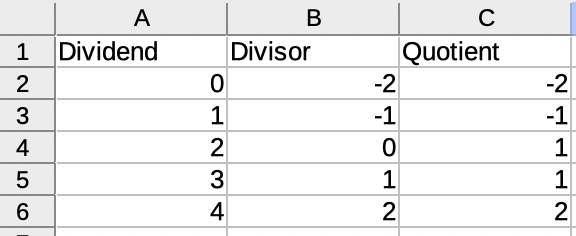
\includegraphics[width=0.9\textwidth]{Exercise1Soln.png}
\end{frame}
\section{Further Reading}
	\begin{frame}
		\frametitle{Further Reading}
		Computer Applications for Life Sciences Chapter 2, p. 15-20
	\end{frame}
\end{document}
